\tcbsection{Support for Student Personal and Academic Growth}

\subsection{C1 Student Connectedness}

\subsubsection{Adequate Personalized Support}

\indicator{The school has available adequate services, including referral services, to support all students in such areas as health, career and personal counseling, and academic assistance.}

\prompt{Evaluate the availability and the adequacy of services, including referral services, to support students in such areas as health, career and personal counseling, and academic assistance.}

\begin{findings}
All seniors are enrolled in Senior Seminar to ensure they have information on graduation requirements, coaching on assembling application portfolios, and choosing target colleges to which they will submit applications.

{\centering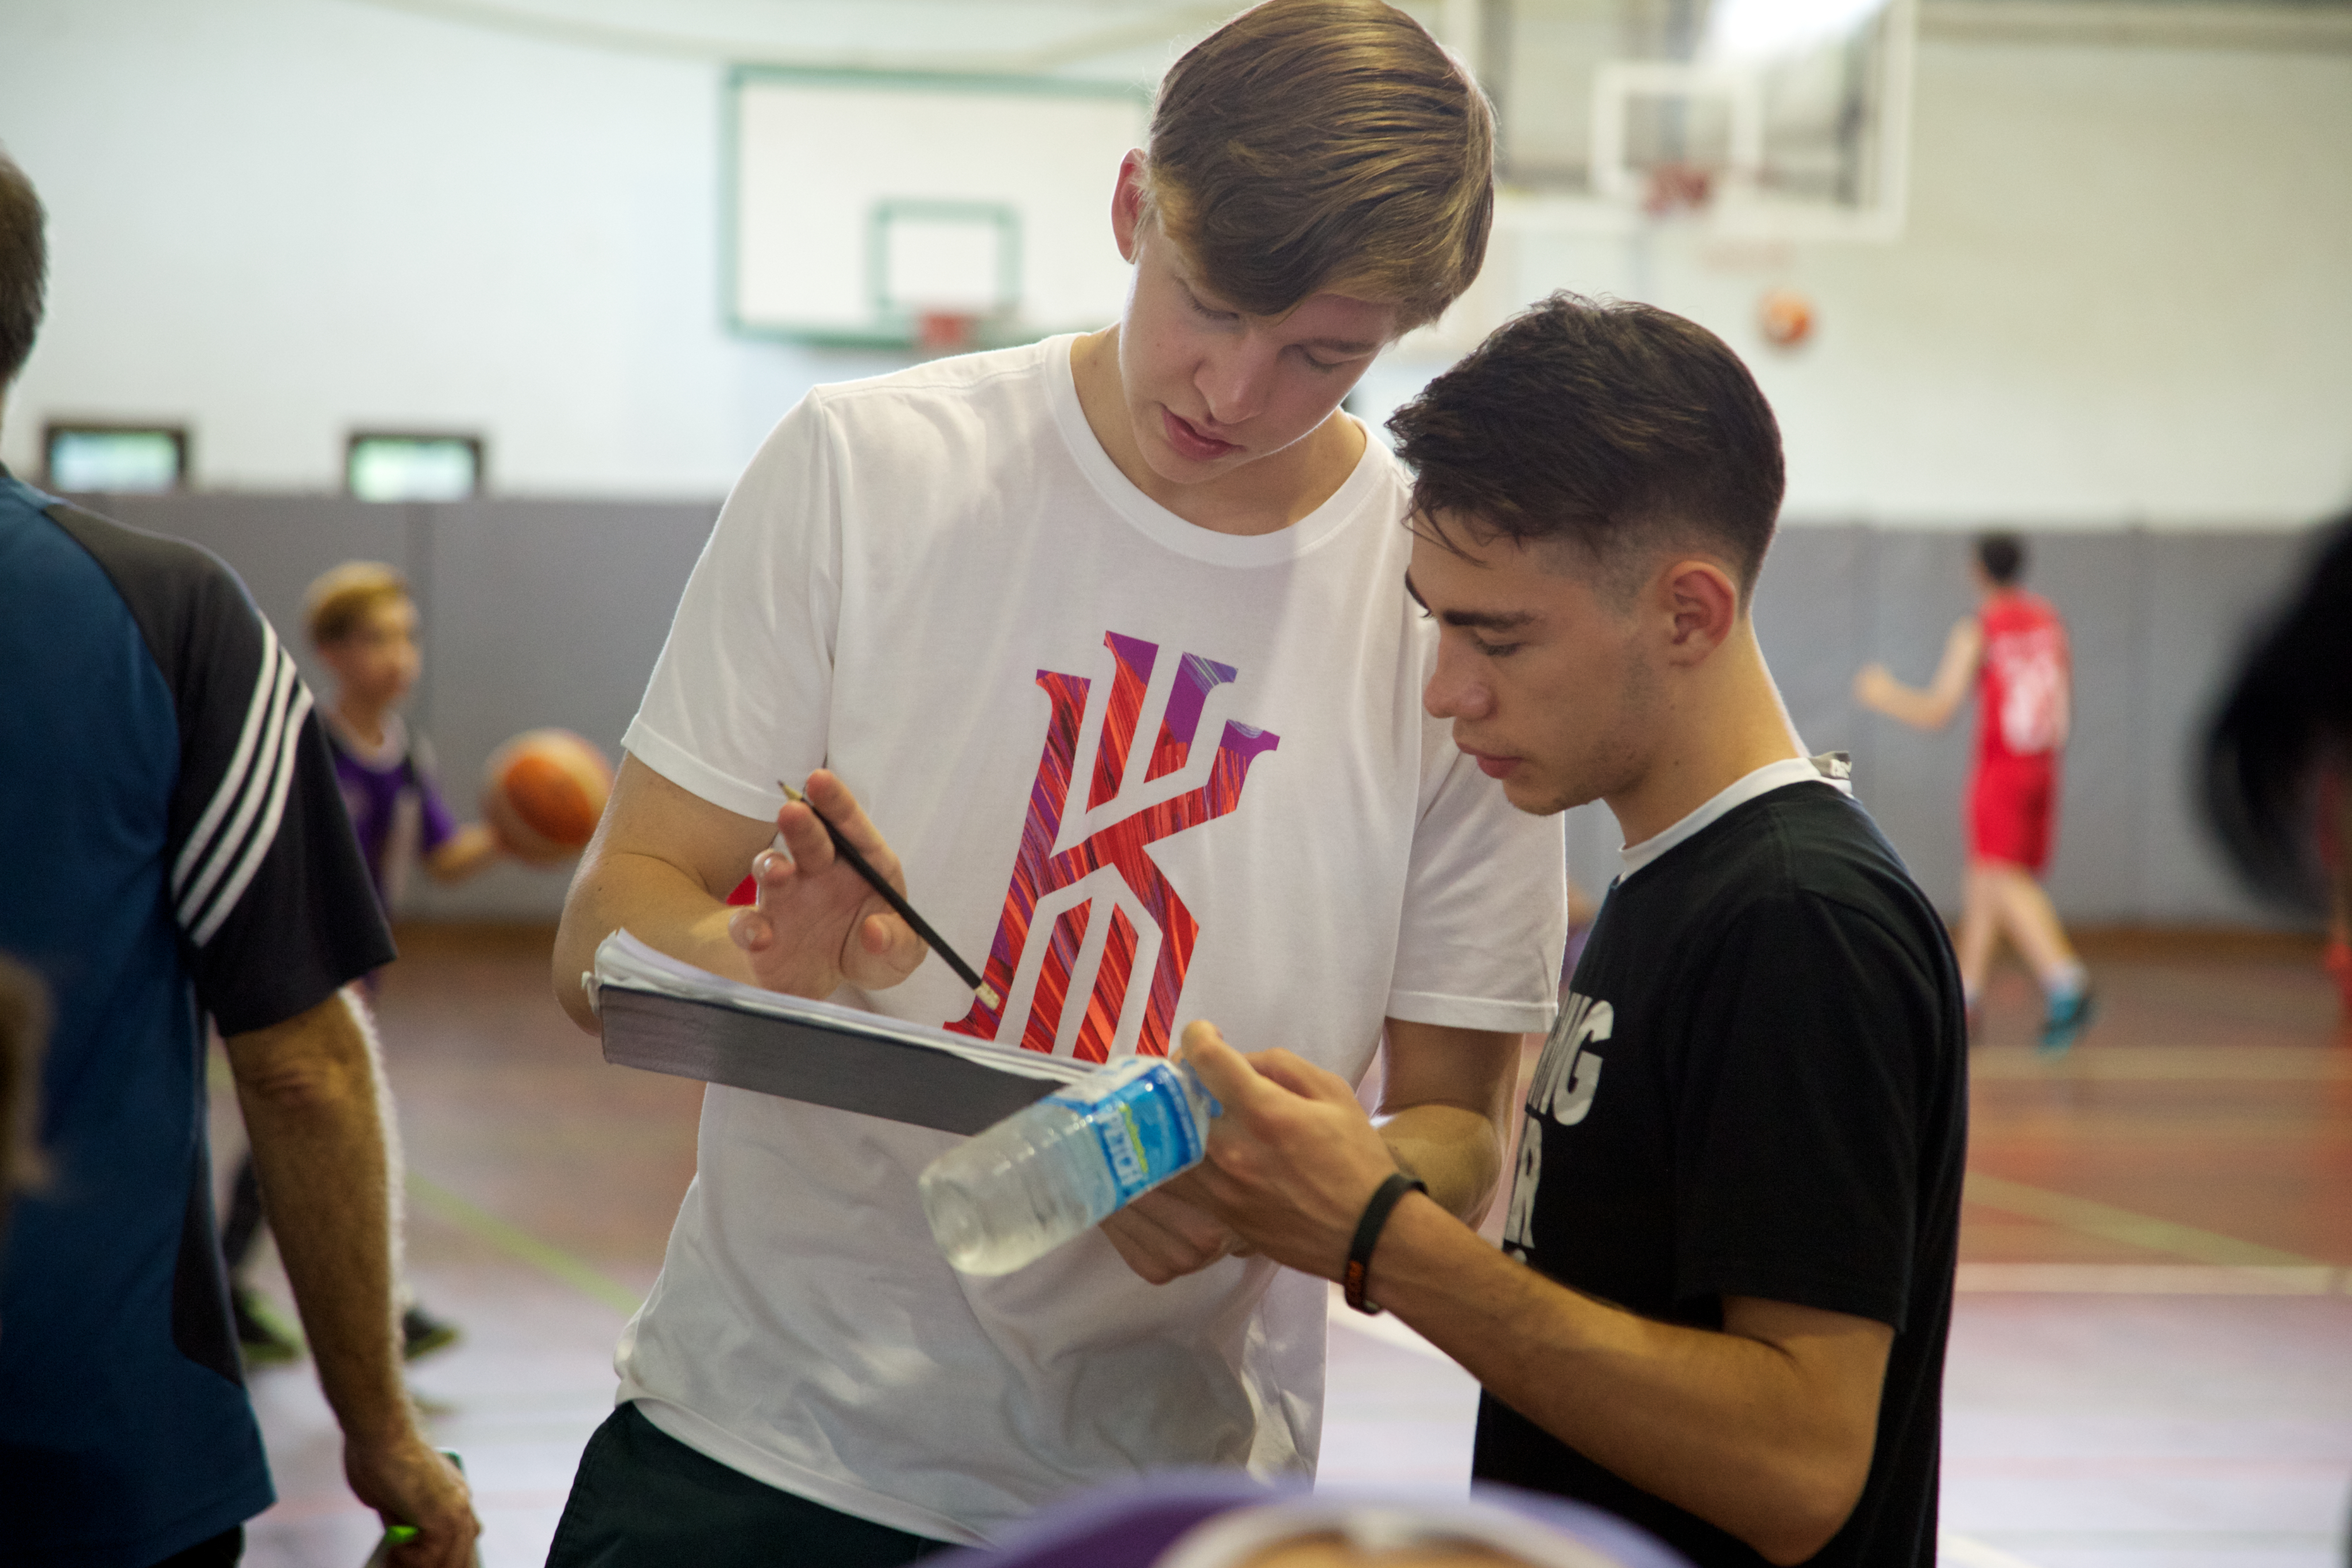
\includegraphics[width=\textwidth]{4_3_1_a.jpg}}

Free after school academic assistance is available grades 3 - 12 on campus throughout the school year. This program allows high school students to earn required community service hours and provides effective peer tutoring for students.  \href{http://blogs.cmis.ac.th/newsletter/2015/09/17/einstein-eagles-starts-monday-get-involved/}{Einstein Eagles Homework Club} is one example of this assistance.

Academic Lab is available to all secondary students on an as-needed basis as well as for students whose need is through regular review of earned grades. A teacher is assigned duty in this room to assist with organization, review assignments, and oversee individualized computer-based foundational skills to all at-risk students. High school students with identified learning needs and English Language learners are placed in a semester-long foundational course called \href{https://drive.google.com/open?id=100aj_4W2p7cnSRhdpkEhTtGRoBIBMe6Uy8JgKBVyofk}{Writing With Style} in order to provide academic assistance. A biweekly review of all MS/HS grades in PowerSchool is done with Department Administrator oversight.

Elementary teachers identify students with specific learning needs through classroom work and DRA reading assessments done twice each school year. Intervention strategies are recommended and implemented in a program of tiered support designed to help teachers differentiate lessons and provide adequate academic assistance that affords all students opportunities to access and meet learning skills and standards. Examples of these are DRA, Strategies and Resources Guide, Elementary ESL teaching in small groups in and out of the classroom, instructional aides assist with teaching in small groups, 1:1 and whole class learning activities in grades pre K - 3, interning student teachers assist with teaching in small groups, 1:1 and whole class learning activities in grades 4 - 5. 

{\centering\includegraphics[width=\textwidth]{4_3_1_b.jpg}}

Individual and group personal counselling sessions are available at all grade levels through the ES, MS and HS counselors. The elementary school counselor visits each class twice monthly to provide support of school wide behavior norms and expectations in our Virtues program and PBIS elementary system; the middle school counselor teaches weekly Wellness classes that address issues of personal development, academic readiness and study skills, community service activities; the high school counselor maintains daily office hours for drop-in and scheduled personal and college/career counselling services, use of the Overgrad planning system for all high school students, reviews all high school students’ schedules to ensure graduation requirements are met and oversees the Senior Seminar class. CMIS also offers a course planning \href{https://docs.google.com/document/d/16eIB9M_ucfMOXqUCxWzIenWzrnKBg2kegjcK8XHlTqI/edit#heading=h.6sft8ugn206j}{handbook}, college visits, college fair days on and off campus, a Korean parents information night and the \href{http://cmis.ac.th/}{School website}.

\begin{itemize}
\item The \href{https://sites.google.com/a/cmis.ac.th/cmis-health-office/home}{CMIS Health Office} implements and communicates school wide wellness initiatives such as immunizations.
\item Provides first aid and emergency care for students in need and first aid cover for extra-curricular activities.
\item Manages communicable diseases within the school and coordinates school response. 
\item Provides annual Health Checks including vision testing, scoliosis exams, weight and height recording. 
\item Reviews health and safety policies and procedures school wide, and manages recording of accidents
\item Oversees cafeteria menu and standards 
\item Tests water quality and manages control of mosquito population. 
\item Manages emergency procedures including fire, evacuation and lockdown drills.
\item Gathers medical information and immunization records for all students and manages students with chronic diseases and allergies through Individualised health-care plans.
\item Provides teachers with health alerts for students with health needs via Powerschool
\item Provides first aid and CPR training to staff and students and provides health-related lessons to elementary school.
\end{itemize}
 
English Language Learners are identified with a standardized test (WIDA) administered on entrance and at the start and end of each school year (WIDA-MODEL) until they are able to demonstrate near-mastery levels of English in the four strands of speaking, listening, reading and writing.  Qualified ESL teachers provide segregated small group skills teaching in pull-out classes as needed as well as in-class assistance and scaffolding for students in grades K-12 so that all students have access to and are able to make progress in our curriculum. The \href{https://docs.google.com/document/d/1j2Z1tLgRgfX9CH3dzoYtU_GOhPOVWKPl6iFlvWqd6wM/edit}{fee schedule} for this support has been changed so that there is a one-time fee paid in a student’s first year at CMIS and all Student Services, including English language supports, are offered at no cost from a student’s second year in our school in order to more effectively provide universally available academic assistance. 

{\centering\includegraphics[width=\textwidth]{4_3_1_c.jpg}}

\href{http://blogs.cmis.ac.th/eagles/faith-service/spiritual-life/}{Spiritual Advisor} position is a paid, full-time position established to implement programs such as \href{http://blogs.cmis.ac.th/eagles/faith-service/spiritual-life/}{Weekly Bible Study Groups}. These programs are open to students of all faiths and address the school’s focus on Christian values and virtues.

\minor{So what...}

CMIS provides a range of support services to serve diverse community and student needs but because not all needs.
\end{findings}

{\centering\includegraphics[width=\textwidth]{chapter4_C1_p1.jpg}}

\subsubsection{School Support Systems}

\indicator{The school coordinates a system of support services that provides for maximum effectiveness, including the processes for intervention and referral. }

\prompt{Is the level of school coordination of the system of support services allowing for maximum effectiveness? Are the processes for intervention or referral effective?}

\begin{findings}
The Student Services Coordinator position was created in 2015 to oversee admissions, identification, referrals, interventions and support services for all students, grades preK -12.

CMIS uses a norm-referenced standardized assessment tool (WIDA) with all student applicants to identify incoming students who may need English language support, learning support services and to monitor program’s effectiveness through regular re-assessments.
 
{\centering\includegraphics[width=\textwidth]{4_3_1_d.jpg}}

We have developed a ‘teacher toolkit’ of applicable classroom interventions such as differentiation techniques, accommodations that promote universal planning, adaptive skills practice, and behavior management protocols. The Student Success Team has also developed a tracking sheet to help teachers identify struggling students and implement intervention strategies in the classroom. Finally, a services flow chart was designed to identify and address student needs.

\minor{So what...}

CMIS has resources available to help teachers more successfully address diverse learners, but teachers need to be made aware of these resources and coaching in the implementation of the resources in their classroom.
\end{findings}

\subsubsection{Strategies Used for Student Growth/Development}

\indicator{Strategies are used by the school leadership and staff to develop personalized approaches to learning and alternative instructional options which allow access to and progress in the rigorous standards-based curriculum. Examples of strategies include: level of teacher involvement with all students, a curriculum that promotes inclusion, processes for regular review of student and schoolwide profiles, and processes and procedures for interventions that address retention and redirection.}

\prompt{Evaluate the effectiveness of the types of strategies used by the school leadership and staff to develop personalized approaches to learning and alternative instructional options which allow access to and progress in the rigorous standards-based curriculum.}

\begin{findings}
High school students who need a personalized course of study to earn credits required for graduation may pursue independent study options that include coaching athletic teams, online courses with US accredited programs or may propose other \href{http://www.ck12.org/}{alternative instructional options}. Students with non-standard academic backgrounds, such as children of missionary families who have been home-schooled, are provided with support to scaffold their access to and progress in our rigorous, standards-based curriculum through programs such as \href{http://www.wilsonlanguage.com/programs/wilson-reading-system/}{Wilson Reading}, \href{https://www.readnaturally.com/}{Read Naturally} or other online curricula.

{\centering\includegraphics[width=\textwidth]{4_3_1_e.jpg}}

All students, including those with identified learning needs and English Language Learners, are placed in general classrooms to the greatest possible extent in order to ensure access to and measurable progress in our standards-based curriculum. Exceptional learners with diagnosed, documented learning needs are placed on a \href{https://drive.google.com/drive/u/0/folders/0B_rFN7xA3AUNdlVaY2E1WGo1bUE}{Student Support Plan}, a \href{https://drive.google.com/drive/u/0/folders/0B_rFN7xA3AUNdlVaY2E1WGo1bUE}{504 Accommodations Plan} or an \href{https://drive.google.com/drive/u/0/folders/0B_rFN7xA3AUNdlVaY2E1WGo1bUE}{Individualized Education Plan} that follow US standards, so that such students can receive Learning Support services if they move to another school or be granted accommodations when taking the SAT or AP examinations. 

Effectiveness is measured by regular reviews of student grades, teacher reports and student self-evaluations.

\minor{So what...}

All CMIS students are challenged to work to their best ability in the general school population but given support as needed but not all staff are aware of all of these options.
\end{findings}

{\centering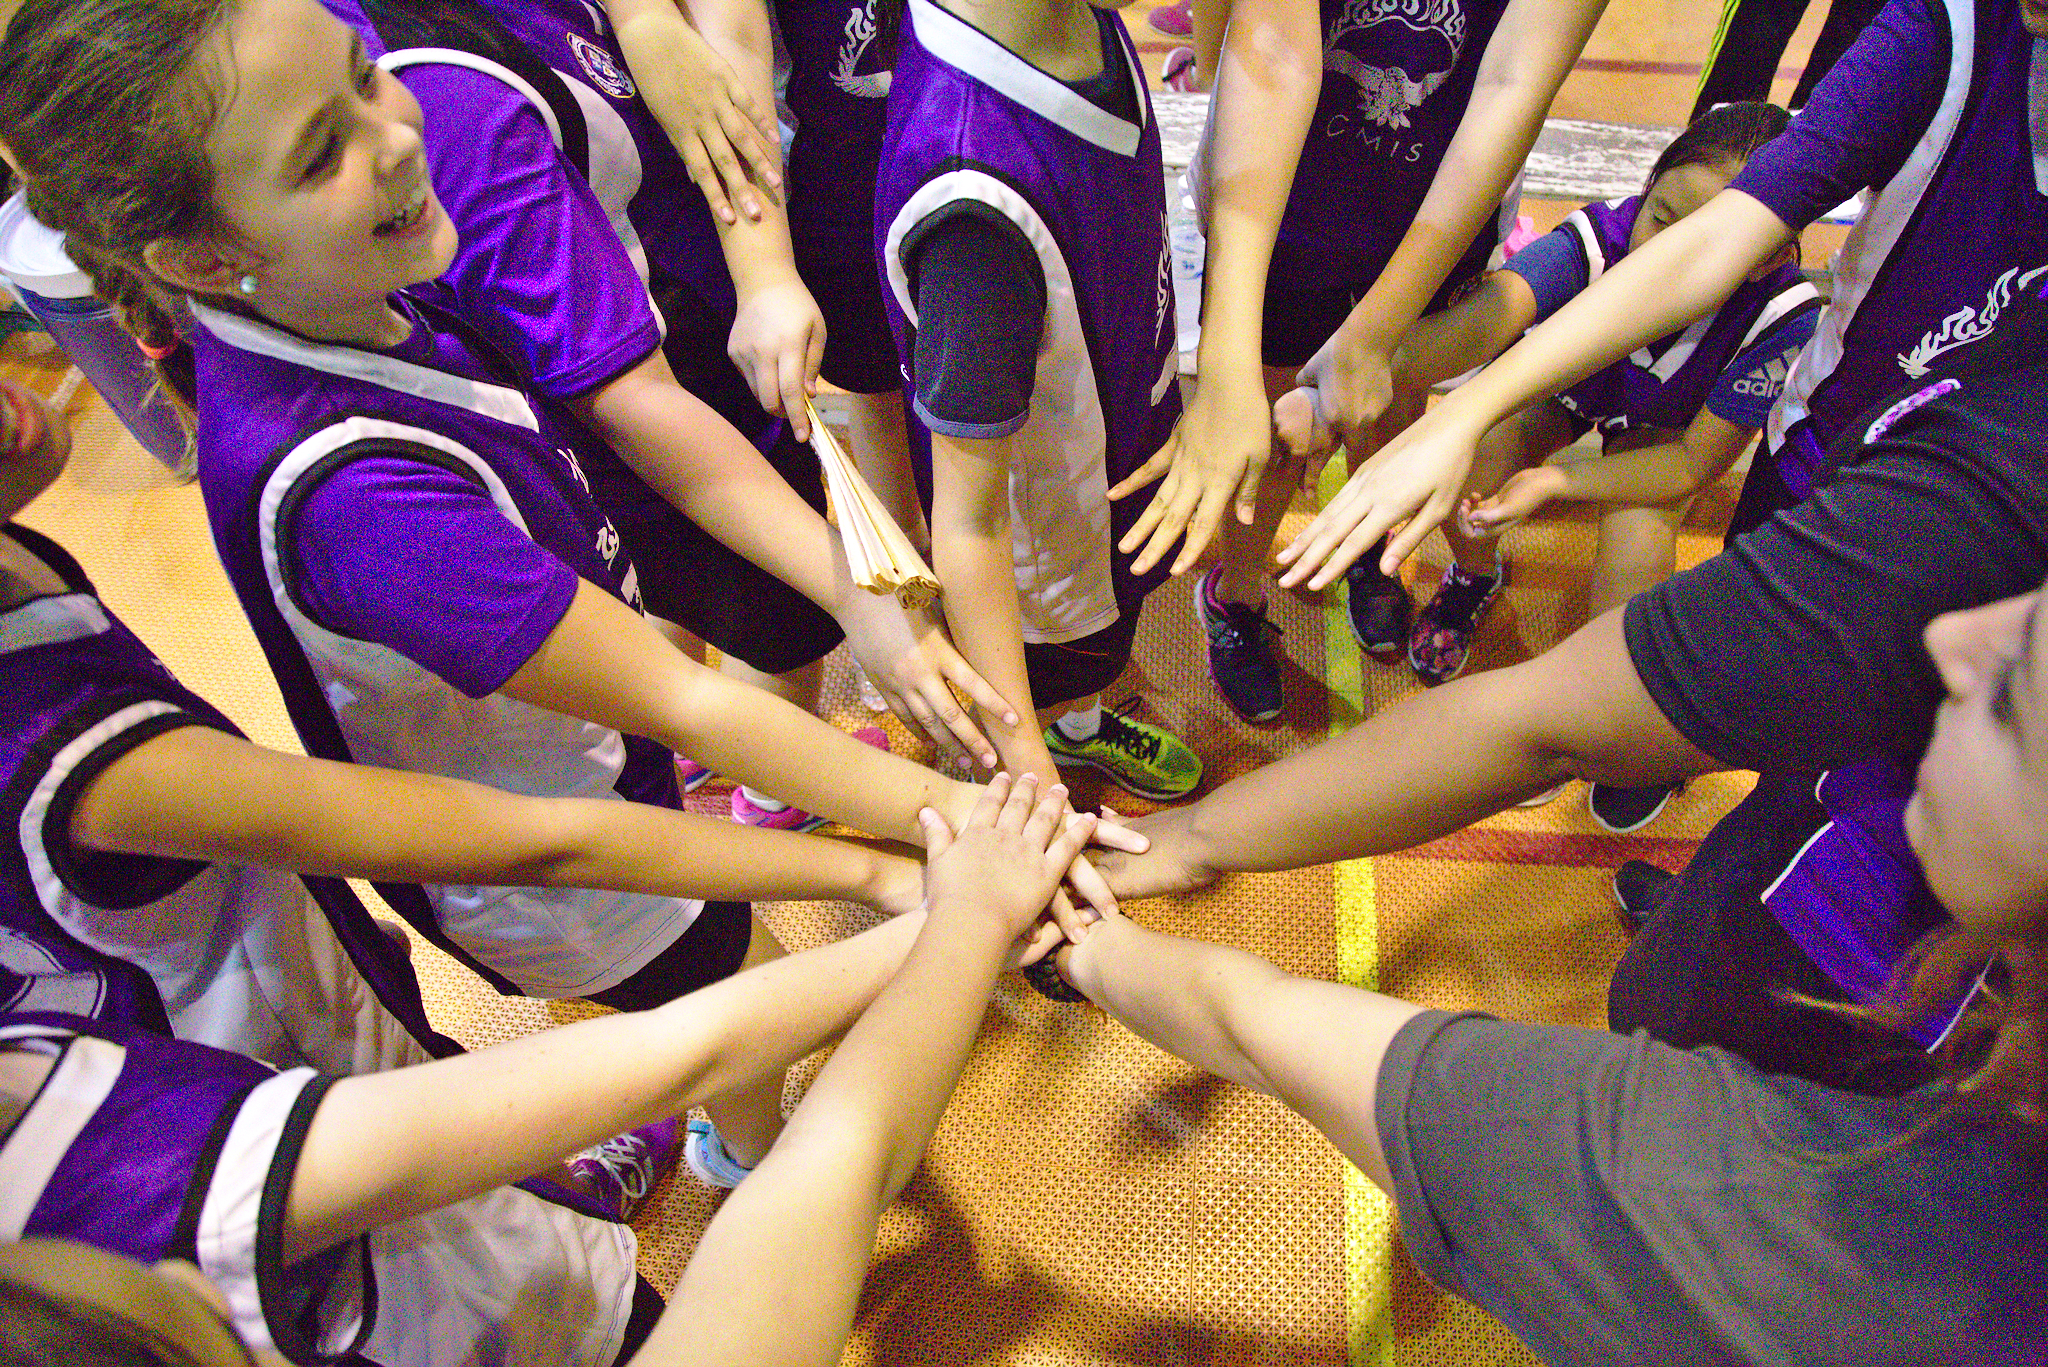
\includegraphics[width=\textwidth]{chapter4_C1_p2.jpg}}

\subsubsection{Support Services and Learning}

\indicator{The school leadership and staff ensure that the support services and related activities have a direct relationship to student involvement in learning, e.g., within and outside the classroom, for all students.}

\prompt{Evaluate the extent to which the school leadership and staff ensure that the support services and related activities have a direct relationship to student involvement in learning, e.g., within and outside the classroom. Evaluate the processes that are used to identify under-performing or struggling students and the interventions to address these identified student learning needs.}

\begin{findings}
All support services, including learning support, counselling services and ESL teaching, provide instruction that is linked to teaching and learning standards used in students’ classrooms and Co-curricular activities. All support services are meant to address clearly identified learning needs and reinforce the values of the \href{http://cmis.ac.th/about/vision}{School Mission Statement}. 

{\centering\includegraphics[width=\textwidth]{4_3_1_f.jpg}}

Students are identified and referred by evaluation of grades, scores on standardized placement tests (WIDA) and teacher evaluations (Power School comments and grades).  Interventions for English Language Learners, struggling or under-performing and gifted students are collaboratively agreed on by teachers, family and school support staff and tailored to address individual needs. Regular progress reports evaluate the effectiveness of the interventions and are shared with the teacher, family and student to assess progress and refine instruction and intervention strategies to better address need.

\minor{So what...}

Though CMIS identifies and provides services for our diverse student population, structures should be developed to more effectively communicate student progress to teachers and parents. 
\end{findings}

\subsubsection{Co-Curricular Activities}

\indicator{School leadership and staff link curricular and co-curricular activities to the academic standards and schoolwide learner outcomes, i.e., global competencies. Students have the opportunity to communicate with diverse audiences locally and worldwide. Students contribute to local and/or global actions and service opportunities.}

\prompt{Evaluate the extent of the availability and link of curricular and co-curricular activities for all students to the academic standards and schoolwide learner outcomes, i.e., the global competencies. How effective are these efforts?}

\begin{findings}
\minor{Background and Timeline on the Development of Student Life at CMIS}

The following timeline makes clear that CMIS has been committed to providing meaningful co-curricular activities for students that have the support and backing of administration and the appropriate faculty/staff resources, time, and expertise to carry out these activities in a way that aligns with the school vision, mission, and student learner outcomes.

\minor{2012-2013}
\begin{itemize}
\item HS/MS Student Council Adviser becomes a 20\% faculty work assignment
\item \href{https://docs.google.com/document/d/1sTrMTOsEmYo4TcWgqYYYepmbt43RhWDNO9Juxo3xS20/edit?usp=sharing}{Athletic Department Philosophy} adopted to align with CMIS Mission and Vision Statement
\item \href{http://blogs.cmis.ac.th/eagles/athletics/}{CMIS Athletics website} launched
\end{itemize}

\minor{2013-2014}
\begin{itemize}
\item \href{http://blogs.cmis.ac.th/eagles/clubs-activities/policies-forms/}{HS/MS Student Organization Foundational Form} adopted
\item HS/MS Student Organization Fair added to the annual \href{http://blogs.cmis.ac.th/eagles/calendars/events-calendar/}{School Events Calendar}
\end{itemize}

\minor{2014-2015}
\begin{itemize}
\item Athletic Director becomes Director of Activities and Athletics, shift from a part-time teaching, part-time admin position to a full-time admin position
\item ES Activities Fair added to the annual \href{http://blogs.cmis.ac.th/eagles/calendars/events-calendar/}{School Events Calendar}
\item Community Service Coordinator/Spiritual Adviser created as a half-time position to provide oversight of community service projects and pursue cooperative service opportunities and activities fostering Christian virtues and respect for diverse faith traditions      
\end{itemize}

\minor{2015-2016}
\begin{itemize}
\item Office of Student Life (OSL) founded to focus on the following “beyond classroom” areas: faith/service, clubs/activities, the arts, and athletics
\item CMIS Athletics website expanded to become \href{http://blogs.cmis.ac.th/eagles/}{Student Life website}
\item HS/MS \href{http://blogs.cmis.ac.th/eagles/clubs-activities/ms-hs/stuco/}{Student Council} structure revised
\item Activities policies, procedures, and forms adopted
\end{itemize}

\minor{2016-2017}
\begin{itemize}
\item Athletic Department budget expanded and revised to be an Office of Student Life budget
\item Community Service Coordinator/Spiritual Adviser position becomes a full-time position
\item HS/MS Student Council Adviser becomes HS/MS Activities Coordinator; HS/MS Activities Coordinator a 20\% faculty work assignment and HS/MS Student Council Adviser an annual stipend assignment
\item Position descriptions adopted with budgetary support:
\begin{itemize}
\item HS/MS Activities Coordinator
\item ES Activities Coordinator
\item MUN Adviser
\item Honor Society Adviser
\item Student Council Adviser
\item Varsity Head Coaches
\item Varsity Assistant Coaches
\item Junior Varsity Coaches
\item MS/ES Coaches
\end{itemize}
\item \href{https://drive.google.com/open?id=1xqBFIjl7jeaT2qJR0Fxga71sfk0juq6pZzDbk8EOibI}{Student Life Handbook} written for first time
\end{itemize}

\minor{Curricular Activities at CMIS}

CMIS school leadership and staff have made an active effort to link curricular activities to the academic standards

\begin{itemize}
\item \href{http://blogs.cmis.ac.th/newsletter/2016/03/16/earth-science-expo-2016-march-30/}{Earth Science Expo}
\item \href{http://blogs.cmis.ac.th/newsletter/2016/03/21/cmis-student-take-top-awards-in-the-south-asia-division-of-the-national-history-day-competition/}{National History Day Competition}
\item \href{http://gallery.cmis.ac.th/2016-2017/Elementary-Sports-Day/}{ES Sports Day}
\item \href{http://gallery.cmis.ac.th/2016-2017/science_waterfall_fieldtrip/}{Class Field Trips}
\item Thai Department HS Field Trip
\end{itemize}

CMIS school leadership and staff have made an active effort to link curricular activities to schoolwide learner outcomes.

\begin{itemize}
\item Courageous Learners
\begin{itemize}
\item \href{http://gallery.cmis.ac.th/2015-2016/graduation/}{Graduation}
\item \href{http://blogs.cmis.ac.th/newsletter/2016/05/12/save-the-date-may-24-hsms-awards-events/}{HS Awards Evening and MS Awards Assembly}
\item 8th Grade Annual Retreat
\item \href{http://gallery.cmis.ac.th/2015-2016/bridging_ceremony/}{ES Bridging Ceremony}
\item ES Assemblies
\end{itemize}
\item Responsible Global Citizens
\begin{itemize}
\item \href{http://blogs.cmis.ac.th/newsletter/2016/11/04/cmis-proud-to-be-a-member-school-of-the-national-honor-society/}{National Honor Society}
\item \href{http://blogs.cmis.ac.th/newsletter/2015/02/18/cmis-thai-day-2015/}{Thai Day}
\item \href{http://blogs.cmis.ac.th/newsletter/2016/02/05/cmis-international-day-friday-february-19/}{International Day}
\item ES Assemblies
\item Virtues Program
\end{itemize}
\end{itemize}

\minor{Co-Curricular Activities at CMIS}

CMIS school leadership and staff have made an active effort to link co-curricular activities to schoolwide learner outcomes
\begin{itemize}
\item Faith/Service
\begin{itemize}
\item  HS Service Hours Requirement
\item  MS Service Trips to Hope House
\item  \href{http://blogs.cmis.ac.th/eagles/faith-service/spiritual-life/}{Weekly Bible Study Groups}
\item  Philosophy Club
\end{itemize}
\item The Arts
\begin{itemize}
\item  \href{https://www.youtube.com/watch?v=x4ScCitmSXU&t=3646s}{HS/MS Music Concerts}
\item  HS Band Festival Trip
\item  \href{https://www.youtube.com/watch?v=_S2R2jLdJOU}{MS Band Festival}
\item  \href{http://gallery.cmis.ac.th/2016-2017/Elementary-Christmas-Concert/}{ES Christmas Show}
\item  \href{http://blogs.cmis.ac.th/newsletter/2016/11/15/upcoming-drama-event-the-best-christmas-pageant-ever/}{Drama Productions}
\item  \href{http://gallery.cmis.ac.th/2016-2017/dance_show/}{Dance Shows}
\item  Visual Art Shows
\item  \href{http://blogs.cmis.ac.th/newsletter/2016/03/15/cmis-art-and-music-show-march-17/}{ES Art and Music Recital}
\item  \href{https://www.youtube.com/watch?v=yG677dWZqpw}{HS/MS Talent Show}
\end{itemize}
\item  Clubs/Activities
\begin{itemize}
\item  \href{http://blogs.cmis.ac.th/eagles/clubs-activities/ms-hs/}{HS/MS Student Organizations}
\begin{itemize}
\item Student-Driven Organizations
\item \href{http://blogs.cmis.ac.th/eagles/clubs-activities/ms-hs/stuco/}{Student Council}
\item \href{http://blogs.cmis.ac.th/newsletter/2016/11/04/cmis-proud-to-be-a-member-school-of-the-national-honor-society/}{National Honor Society}
\item \href{http://gallery.cmis.ac.th/2016-2017/MUN/}{Model United Nations}
\item History Bowl
\item Art Club
\item Music Clubs
\item Fencing Club
\item Dance Club
\item Boy Scouts
\end{itemize}
\item \href{http://blogs.cmis.ac.th/eagles/clubs-activities/es/}{Elementary ECAs}
\begin{itemize}
\item Adviser Organized Clubs
\item Chess Club
\item Gymnastics Club
\item Music Club
\item \href{http://gallery.cmis.ac.th/2016-2017/respect_the_beat/}{Dance Club}
\item \href{http://blogs.cmis.ac.th/newsletter/2016/09/16/cub-scouts-returning-to-cmis/}{Cub Scouts}
\end{itemize}
\item \href{http://blogs.cmis.ac.th/eagles/athletics/}{Athletics}
\begin{itemize}
\item Grade 1-12 Athletic Programs, Teams, Practices, and Competitions
\item HS Athletic Team Trips
\end{itemize}
\item Other
\begin{itemize}
\item Christmas and Easter Assemblies
\item Senior Trip
\item MS Teambuilding Activities/Trips
\end{itemize}
\end{itemize}
\end{itemize}

\minor{Students Communicating with Diverse Audiences}

Students at CMIS have the opportunity to communicate with  diverse audiences locally and globally and to contribute to local and global actions and service opportunities.

\minor{Locally}
\begin{itemize}
\item MS Service Trips
\item Thai Department HS Field Trip
\item Thai Day
\item MS Service Trips to Hope House
\item HS Community Service Requirement
\item \href{https://www.youtube.com/watch?v=3Mb6RadmBkA}{Teacher Appreciation Day}
\item \href{http://blogs.cmis.ac.th/newsletter/2015/05/08/cmis-sala-sale-saturday-may-16th/}{Sala Sale}
\item Regular Fundraising Efforts for Communities in Need
\begin{itemize}
\item \href{http://blogs.cmis.ac.th/newsletter/2016/06/07/wow-thank-you-for-your-donations-pitakkiat-school-chiang-rai-update/}{Chiang Rai School Devastated by Fire}
\item \href{http://blogs.cmis.ac.th/newsletter/2016/11/07/angel-tree-project-2016-help-make-christmas-better-for-children/}{Angel Tree} - Christmas Gifts and Winter Clothes Drive for Local Orphans
\item MS T-Shirt Design Contest and Fundraising for Local Orphanage
\end{itemize}
\end{itemize}

\minor{Worldwide/Global}
\begin{itemize}
\item \href{http://blogs.cmis.ac.th/newsletter/2016/03/21/cmis-student-take-top-awards-in-the-south-asia-division-of-the-national-history-day-competition/}{National History Day Competition and Trip}
\item Athletic Trips
\item Band Festival Trips
\item \href{http://blogs.cmis.ac.th/newsletter/2016/02/05/cmis-international-day-friday-february-19/}{International Day}
\item Visiting Author
\item \href{http://gallery.cmis.ac.th/2016-2017/MUN/}{MUN Conferences}
\item College Visits and College Fairs
\item HS Community Service Requirement
\item Fundraising Efforts for Communities in Need
\begin{itemize}
\item \href{http://blogs.cmis.ac.th/newsletter/2015/06/05/elementary-school-fundraiser-for-nepal-raises-30000-baht/}{Nepal Earthquake Response Fundraiser}
\item\href{http://blogs.cmis.ac.th/newsletter/2014/02/07/cmis-fundraising-for-typhoon-haiyan-victims/}{ Philippines Typhoon Response Fundraiser}
\end{itemize}
\end{itemize}

\minor{So what...}

CMIS offers a wide variety of extracurricular activities that are closely linked to schoolwide learning outcomes for all levels (K-12) but these ECAs could be more closely linked to academic standards and participation in sports activities should be more closely linked to GPA requirements.
\end{findings}

\subsubsection{Student Involvement in Curricular/Co-Curricular Activities}

\indicator{The school has an effective process for regularly evaluating the level of student involvement in curricular/co-curricular activities and student use of support services. This includes students involved in projects on global issues, joining networks, and exchanges.}

\prompt{Comment on the effectiveness of the school process for regularly evaluating the level of student involvement in curricular/co-curricular activities and student use of support services.}

\begin{findings}
\minor{Student Involvement in Curricular Activities}

CMIS has processes in place to regularly evaluate the level of student involvement in curricular activities.  Each of these curricular activities has a formalized process for student selection and participation:

\begin{itemize}
\item Graduation
\item Honor Society Selection Process
\item PTG Senior Scholarship Application Process
\item HS Awards Evening and MS Awards Assembly
\item ES Bridging Ceremony
\end{itemize}

\minor{Student Involvement in Co-Curricular Activities}

CMIS has processes in place to regularly evaluate the level of student involvement in co-curricular activities.  Each of these co-curricular activities has a formalized process for student selection and participation.

\begin{itemize}
\item Clubs/Activities
\begin{itemize}
\item Student Council Election Process
\item \href{https://docs.google.com/document/d/10A10VbcdEcStSu9a4tbO-ZsZ38OyqRVfdQH9v1x6\_PI/edit?usp=sharing}{HS/MS Student Org Fair, Sign Up, and Founding Process}
\item ES Activities Fair and  Sign Up Process
\end{itemize}
\item Faith/Service
\begin{itemize}
\item Process for Tracking of HS Community Service Hours
\end{itemize}
\item Athletics
\begin{itemize}
\item Process for \href{http://blogs.cmis.ac.th/eagles/athletics/registration/}{Registering for Athletics Programs}
\item \href{http://blogs.cmis.ac.th/newsletter/2016/06/07/cmis-athletics-2015-2016-review-and-2016-2017-update/}{End of Year Athletics Report} Summarizing Participation
\end{itemize}
\end{itemize}

\minor{Student Use of Support Services}

CMIS has processes in place to regularly evaluate the level of student use of support services.  Each of these support services has a formalized process for evaluating student use.

\minor{So what...}

CMIS offers a wide range of services but needs to institute a means of monitoring the school community’s level of knowledge about and satisfaction with those services.
\end{findings}

{\centering\includegraphics[width=\textwidth]{chapter4_c1_p3.jpg}}

\subsubsection{Student Perceptions}

\indicator{The school is aware of the student view of student support services through such approaches as interviewing and dialoguing with student representatives of the school population.}

\prompt{Comment on the student view of student support services after interviewing and dialoguing with student representatives of the school population.}

\begin{findings}
Students participated in a survey and results showed that they are generally aware that services such as tutoring, extracurricular activities, sports, community service and counselling are available but are not uniformly confident about who the services are for and when they are able to access those services.

{\centering\includegraphics[width=\textwidth]{4_3_1_g.jpg}}

\minor{So what...}

CMIS offers a range of services but needs to regularly remind the school community of what services are available through means such as wider advertising of available services through the school website, PTG meetings, weekly principal’s communications with teachers and an information sheet made available in the counsellor’s office and new student information pack
\end{findings}

\subsection{C2 Parent/Community Involvement}

\subsubsection{Regular Parent Involvement}

\indicator{The school implements strategies and processes for the regular involvement of parents and the community, including being active partners in the learning/teaching process for all programs. The school involves non-English speaking parents and/or online parents.}

\prompt{Evaluate the strategies and processes for the regular involvement of parents and the community, including being active partners in the teaching/learning process. Comment on the effectiveness of involving non-English speaking parents and/or online parents.}

\begin{findings}
CMIS implements strategies and processes for the regular involvement of parents and the community as active partners in the learning/teaching processes.

{\centering\includegraphics[width=\textwidth]{4_3_2_a.jpg}}

CMIS strives to provide communication in English, Thai, and Korean for our parent communities and important correspondence is often translated into all three languages.  In 2015, a CMIS community member volunteered their time to be a liaison for the Korean parent community.  Because of the value of this experience, administration hired a part-time Korean Liaison position for the 2016-2017 academic year.

The \href{http://blogs.cmis.ac.th/ptg/}{CMIS parent community} is regularly involved in learning activities on campus, including hosting cultural booths at International Day, being coaches for athletics teams, supporting athletics, drama, and music through “booster clubs”, attending Love and Logic workshops, and attending Family Teacher Conferences.

{\centering\includegraphics[width=\textwidth]{4_3_2_b.jpg}}

In the digital realm, parents are participants in the learning of their sons/daughters through the \href{https://cmis.powerschool.com/public/}{PowerSchool parent portal} and the use of classroom blogs and websites.

\minor{So what...}

CMIS parents and families can join the library, prayer groups, a drama boosters club, and after school music groups in addition to our active Parent Teachers Group but we need to better involve parents in child’s learning so that they feel informed about our standards and expectations.
\end{findings}

{\centering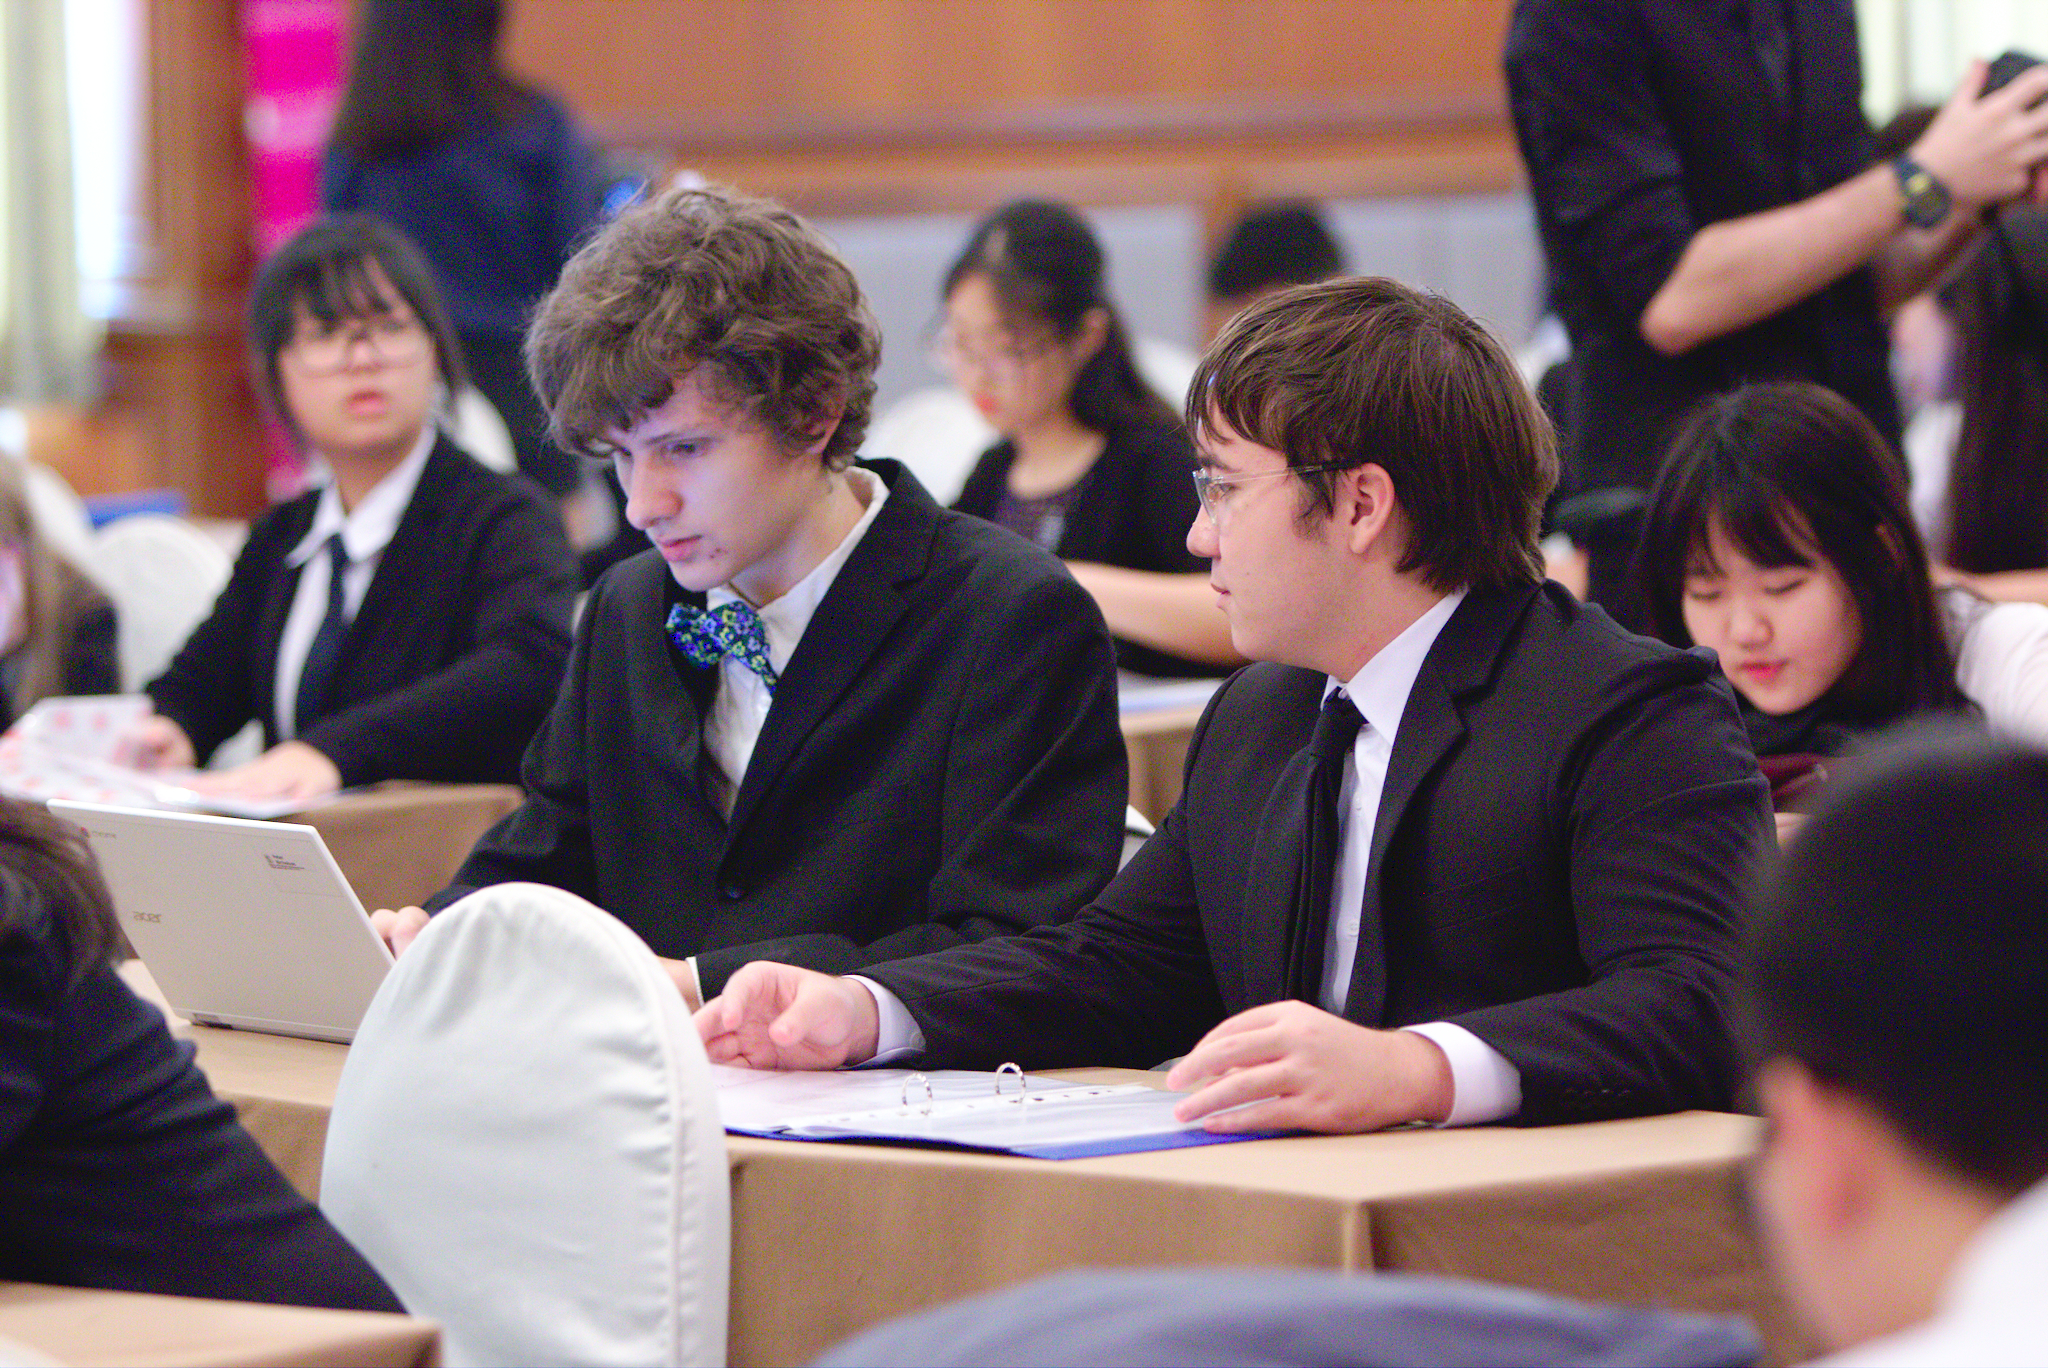
\includegraphics[width=\textwidth]{chapter4_C2_p1.jpg}}

\subsubsection{Use of Community Resources}

\indicator{ The school uses community resources of the host country to support students such as professional services, partnerships, speakers, etc.}

\prompt{How effective is the school use of community resources to support students?}

\begin{findings}
CMIS uses community resources of the host country to support students. CMIS maintains a current listing of \href{https://drive.google.com/drive/u/0/folders/0B_rFN7xA3AUNTC0yaWxCMEVYTkE}{service providers} for students and families, focused on therapeutic treatments and services for emotional, behavioral, and physical issues.

{\centering\includegraphics[width=\textwidth]{4_3_2_c.jpg}}

When appropriate, CMIS invites outside people and organizations to be a part of school curricular and co-curricular events and activities.  Local Rotary club members were invited to be judges for National History Day.  The local Education USA office attends Senior Seminar classes in first semester to support grade 12 students with their college applications. Our \href{http://blogs.cmis.ac.th/ptg/}{PTG} is another means of community outreach and communication. 

{\centering\includegraphics[width=\textwidth]{4_3_1_h.jpg}}

CMIS has many important institutional relationships that support student learning.  As a subsidiary of the Church of Christ of Thailand (CCT), CMIS is able to maintain positive relationships with sister organizations within CCT, including local Thai schools and universities, hospitals, and charitable organizations including a Christmas Gift Drive and support of Hope House, a local orphanage.  Similarly, as the school of choice for U.S. Consulate families and school for various other countries’ consular families, CMIS is able to provide unique opportunities for students to support their learning.

\minor{So what...}

CMIS students are exposed to opportunities to demonstrate Christian values and practice college-readiness skills but maintaining and expanding relationships within the larger Chiang Mai community will create more opportunities for students to develop their strengths
\end{findings}

\subsubsection{Parents/Community and Student Achievement}

\indicator{The school ensures that the parents and school community understand student achievement of the academic standards/schoolwide learner outcomes through the curricular/co‑curricular program. The school works with the parents to help them understand the focus on global competencies and their involvement as partners in the learning.}

\prompt{Determine the adequacy and effectiveness of the school’s strategies to ensure that parents and school community understand student achievement of the academic standards/schoolwide learner outcomes through the curricular/co-curricular program. Evaluate the understanding level and involvement of parents in the focus on students demonstrating global competencies.}

\begin{findings}
\begin{itemize}
\item Elementary and Middle School fundraisers to support charity drives - community service component
\item Korean parents provided with translated information on services made available by Student Services 
\item MS/HS academic and athletic awards and fine arts awards
\item Student of the month community service awards 
\item \href{https://cmis.powerschool.com/public/}{PowerSchool}
\item Curriculum presentation to \href{http://blogs.cmis.ac.th/ptg/}{PTG}
\item Back to School night presentations
\item Parent-Teacher conferences 
\item PTG coffee mornings
\item Elementary newsletters
\item Secondary teacher blogs/websites/Google classroom
\item Classroom displays, assemblies
\item Great Kindness Challenge for whole school
\item \href{https://www.facebook.com/cmis.th/}{Facebook page}
\end{itemize}

{\centering\includegraphics[width=\textwidth]{4_3_2_d.jpg}}

\minor{So what...}

CMIS makes information available in many venues and media but should work to be sure that expectations (such as Student Learner Outcomes) are regularly and consistently explained to all members of our school community
\end{findings}

{\centering\includegraphics[width=\textwidth]{chapter4_C2_p2.jpg}}

\subsubsection{Conclusions}

\begin{findings}
The findings suggest that CMIS addresses this criterion to a high degree.

\minor{Maintain and Monitor}
\begin{itemize}
\item Support positions to addressing identified areas of need (Spiritual Advisor, Korean Community Liaison, Student Services Coordinator).
\item Norm-referenced, standardized tests administration to all CMIS applicants to better identify needs of English Language Learners in all grades.
\item Student services online referral form to ensure consistent implementation of interventions, support plans and services.
\item Counseling positions for elementary, middle and high school as full-time, staffed positions.
\item Access of classroom teachers to a range of supports from Student Success team.
\end{itemize}

\minor{Continue to Improve}
\begin{itemize}
\item More comprehensive identification of individual students who are under-challenged and need  extension opportunities in different curricular areas.
\item Further development of online resources accessible by classroom teachers to support students in the classroom in order to reduce time out of class on remedial or foundation teaching.
\item Communicating availability of services and services offered to students, parents and teachers.
\end{itemize}
\end{findings}
